\documentclass[11pt]{beamer}
\usepackage[utf8]{inputenc}
\usepackage[T1]{fontenc}
\usepackage{lmodern}
\usepackage[english]{babel}
\usepackage{subcaption}
\usepackage{amsmath}
\usepackage{amsfonts}
\usepackage{amssymb}
\usepackage{graphicx}
\graphicspath{{figures/}}
\usetheme{Hannover}

\AtBeginSection[]
{
	\begin{frame}
		\frametitle{Table of Contents}
		\tableofcontents[currentsection]
	\end{frame}
}


\begin{document} 
	\author{Ignacio Condés Menchén}
	\title{Embedded Solution for Person Identification and Tracking}
	\subtitle{Master in Telecommunication Engineering}
	\logo{
\includegraphics[height=1.5cm]{Portada_Logo.png}}
	\institute{Escuela Politécnica Superior\\
		Universidad Carlos III de Madrid}
	\date{July 23, 2020}
	%\subject{}
%	\setbeamercovered{transparent}
%	\setbeamertemplate{navigation symbols}{}

% COVER 
\begin{frame}[plain]
	\maketitle
\end{frame}

% TOC
\begin{frame}
	\frametitle{Table of Contents}
	\tableofcontents
\end{frame}

% 1.- INTRODUCTION
\section{Introduction}
%% Motivation
\subsection{Motivation}
\begin{frame}
	\frametitle{Motivation}
		\begin{columns}
			\column{0.6\textwidth}
			Strong evolution in computer vision research and development.\\
			\vspace{0.2cm}
			Notable spreading of \textit{deep learning} techniques on computer vision: CNNs (\textit{Convolutional Neural Networks}).\\
			\vspace{0.8cm}			
			Multiple applications:
			\begin{itemize}
				\item Autonomous driving
				\item Medical diagnosis
				\item Surveillance
			\end{itemize}
			\column{0.4\textwidth}
			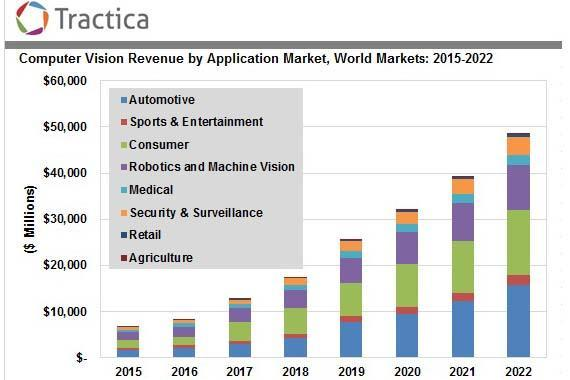
\includegraphics[width=\linewidth]{cv_forecast_2022} \\
			\vspace{0.5cm}
			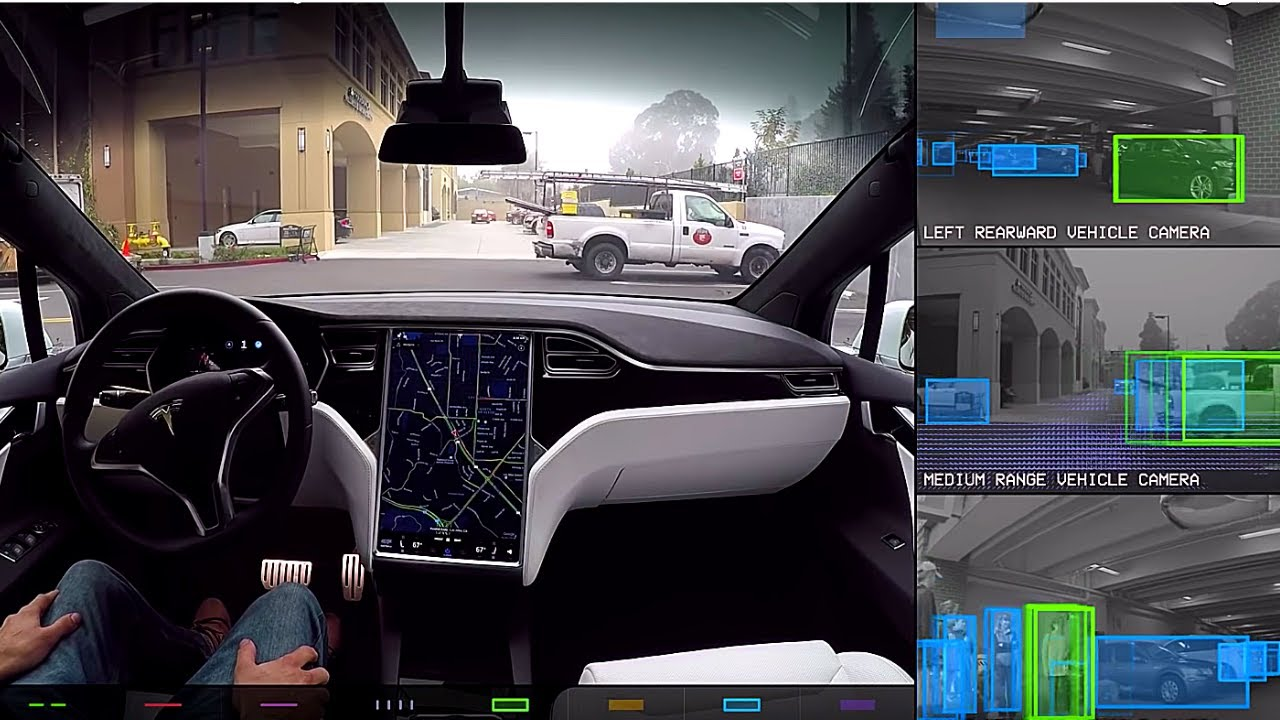
\includegraphics[width=\linewidth]{tesla_autonomous_driving}
		\end{columns}
\end{frame}

\begin{frame}
	\frametitle{Motivation}
		\begin{columns}
			\column{0.5\textwidth}
			Powerful applications in robotics as well:
			\begin{itemize}
				\item Remote inspections on hazardousness
				\item Precision surgery
				\item Social robotics
			\end{itemize}
			\column{0.5\textwidth}
			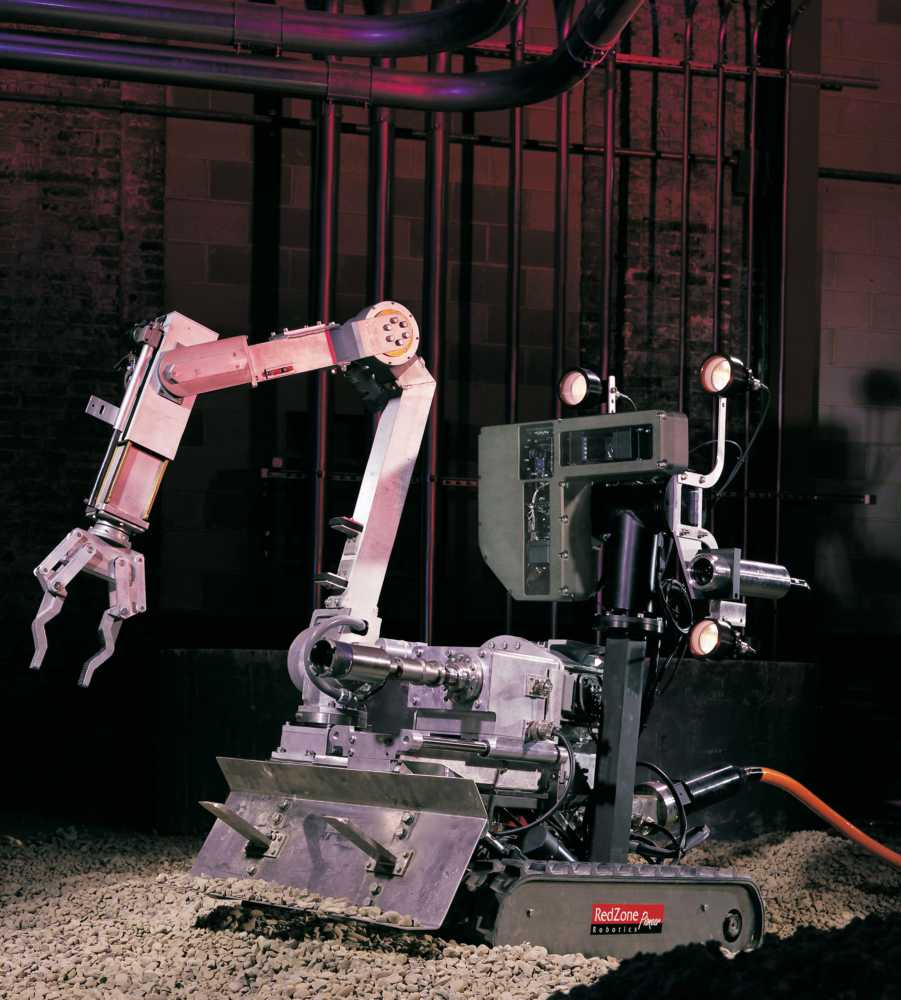
\includegraphics[width=0.5\linewidth]{pioneer_chernobyl} \\
			\vspace{0.5cm}
			\hfill
			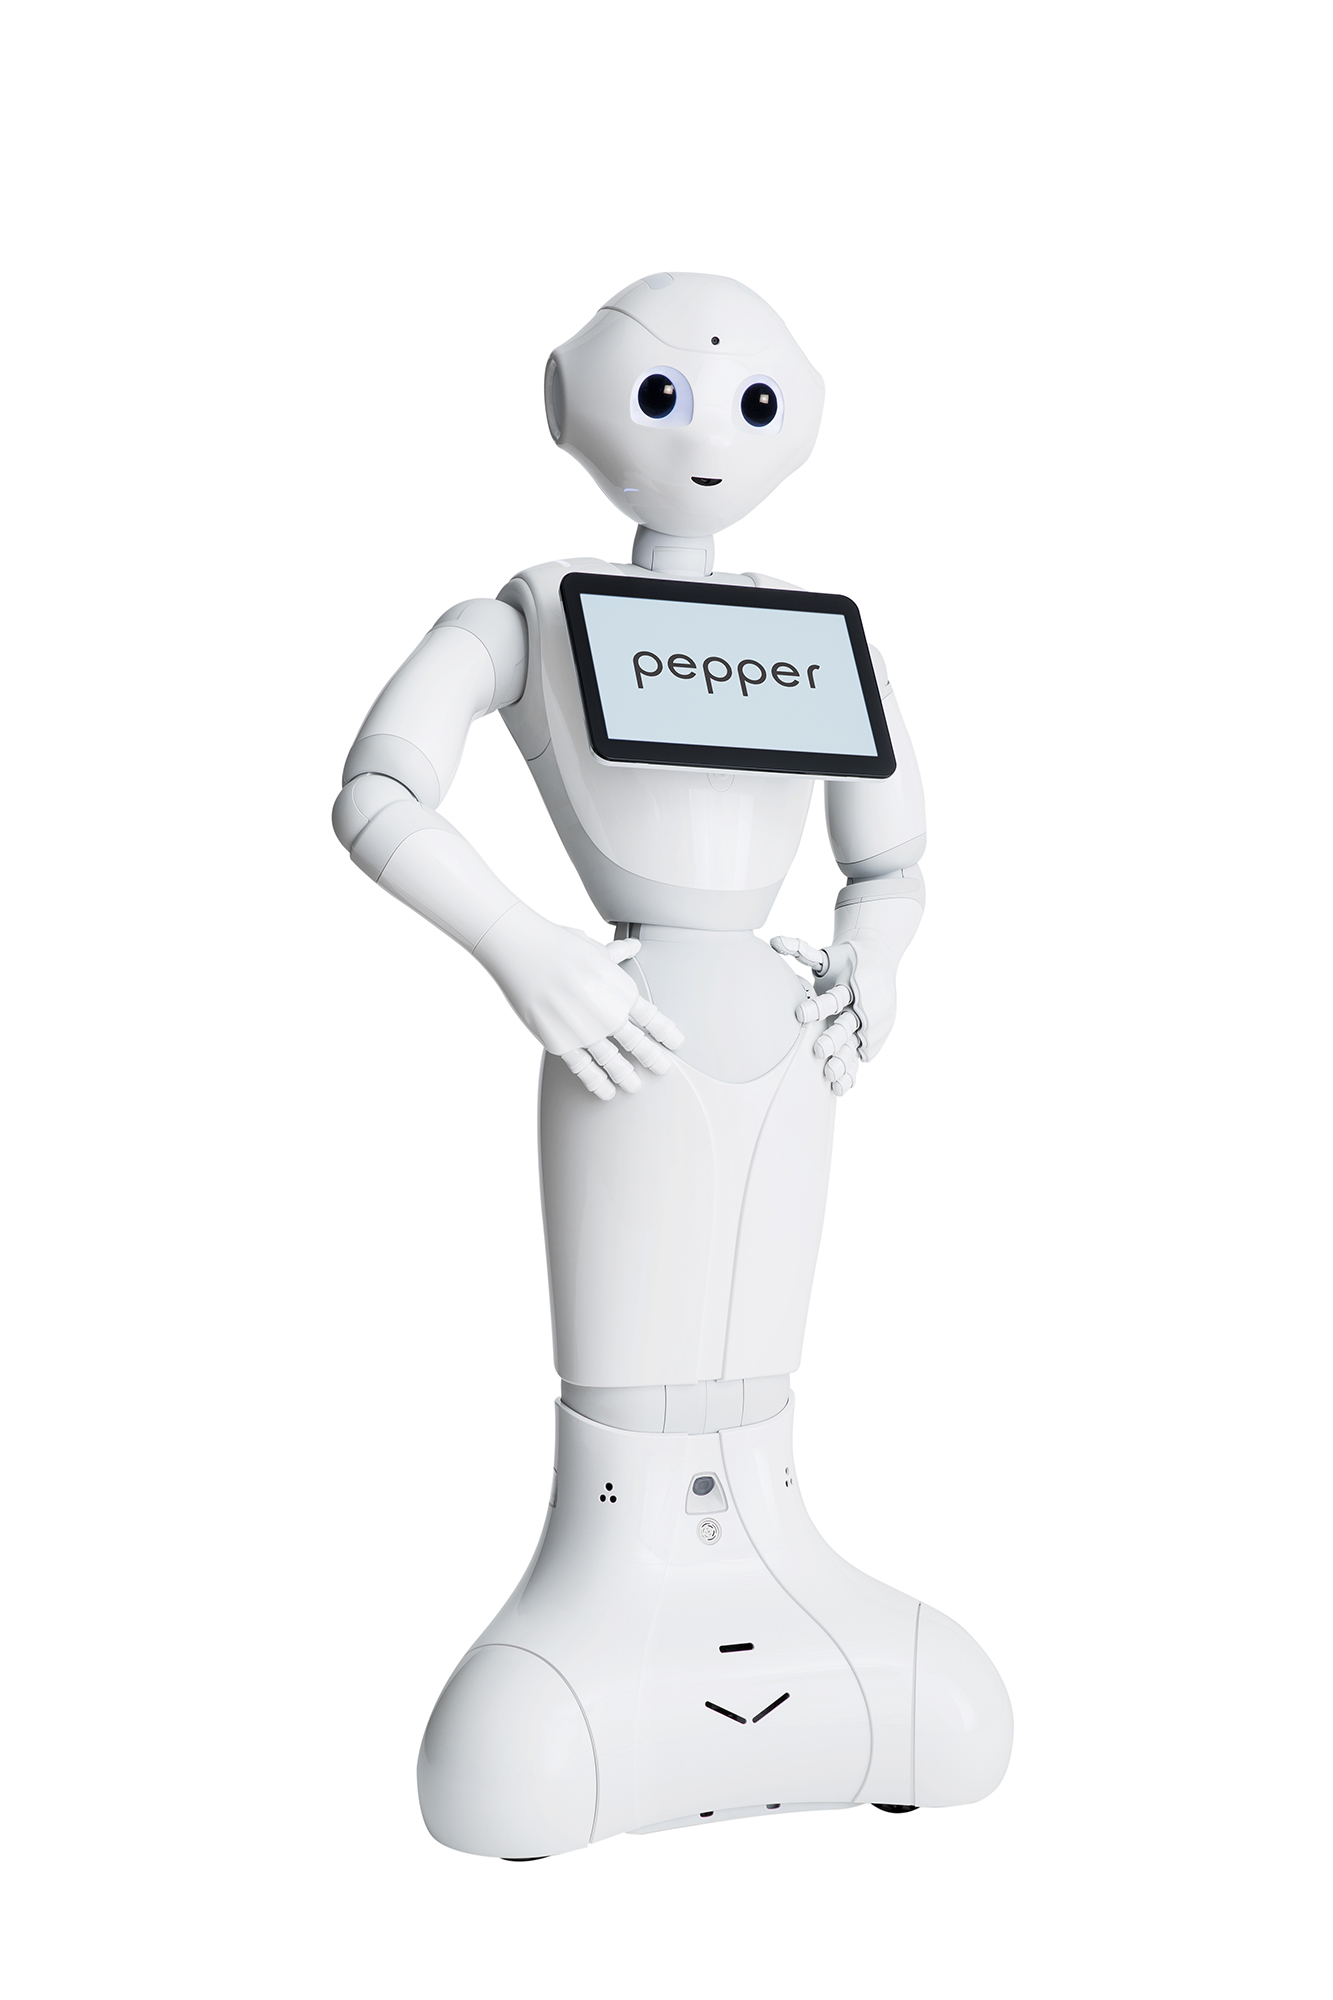
\includegraphics[width=0.5\linewidth]{pepper}
		\end{columns}
\end{frame}

%% Objectives
\subsection{Objectives}
\begin{frame}
	\frametitle{Main goal}
	\begin{columns}
		\column{0.5\textwidth}
		These fields can be combined for programming more intelligent robots.\\
		\vspace{1cm}
		
		This has been pursued in this research: build an \alert{autonomous robot that robustly follows a person}.
		
		\column{0.5\textwidth}
		\vspace{4cm}
		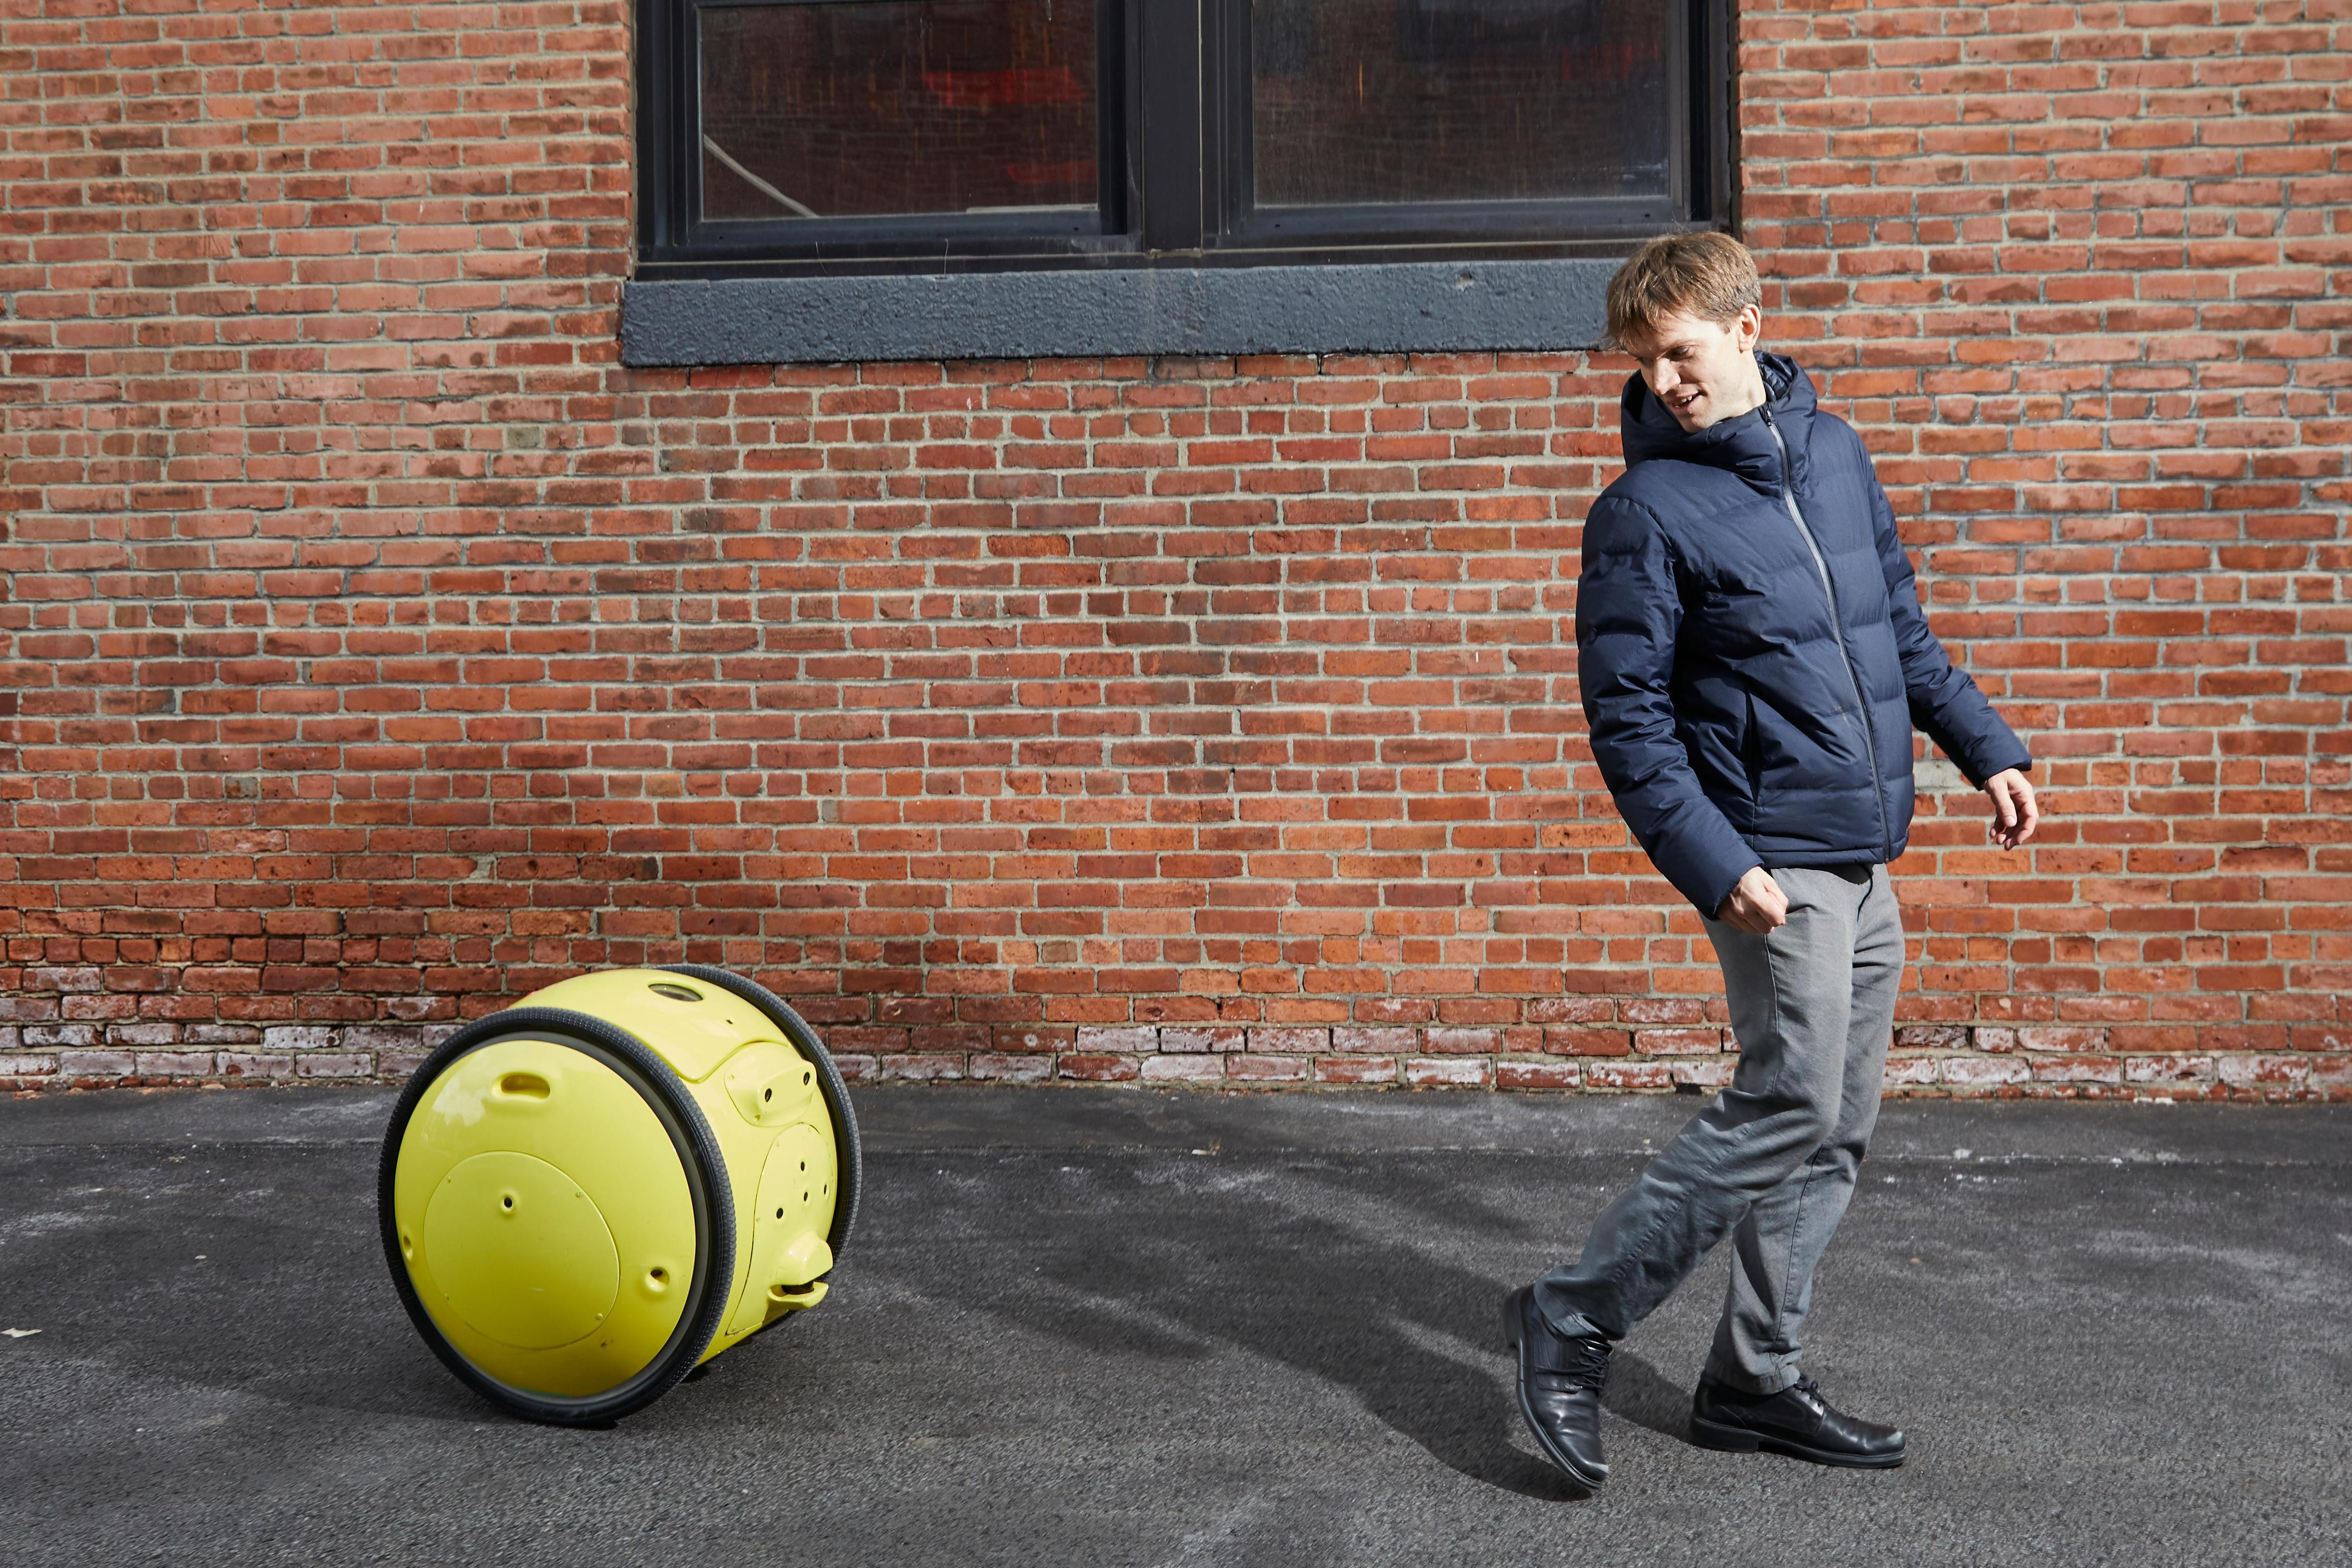
\includegraphics[width=\linewidth]{robot_following} \\
	\end{columns}
\end{frame}

\begin{frame}
	\frametitle{Objectives}
	This goal requires several objectives to be achieved:\\
	\vspace{0.3cm}
	\begin{itemize}
		\item Implement a real-time person following behavior on affordable hardware.
		\item Use only CNNs for the inference tasks.
		\item Enhance the robustness combining the CNNs with optical tracking.
	\end{itemize}
\end{frame}

% Existing techniques
\section{Existing techniques}

%% Person detection
\subsection{Person detection}
\begin{frame}
	\frametitle{Person detection}
		\begin{columns}
		\column{0.40\textwidth}
		\vspace{-0.2cm}
		\begin{itemize}
			\item Viola-Jones detector (adapted from a face detection task) \cite{violajones}.
			\vspace{0.3cm}
			\item HoG (\textit{Histogram of Gradients}) detector \cite{hog_detection}.
			\vspace{0.7cm}
			\item Deep-learning-based detectors: CNNs \cite{alexnet}.
		\end{itemize}
		
		\column{0.60\textwidth}
		\begin{center}
		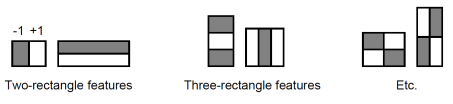
\includegraphics[width=0.9\linewidth]{haar_feats} \\
		\vspace{0.5cm}
		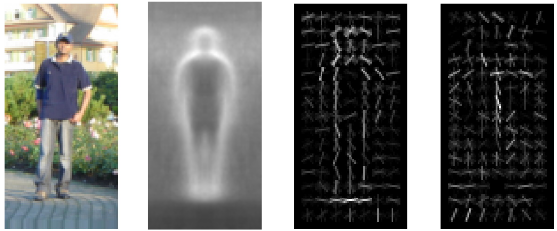
\includegraphics[width=0.7\linewidth]{hog} \\
		\vspace{0.4cm}
		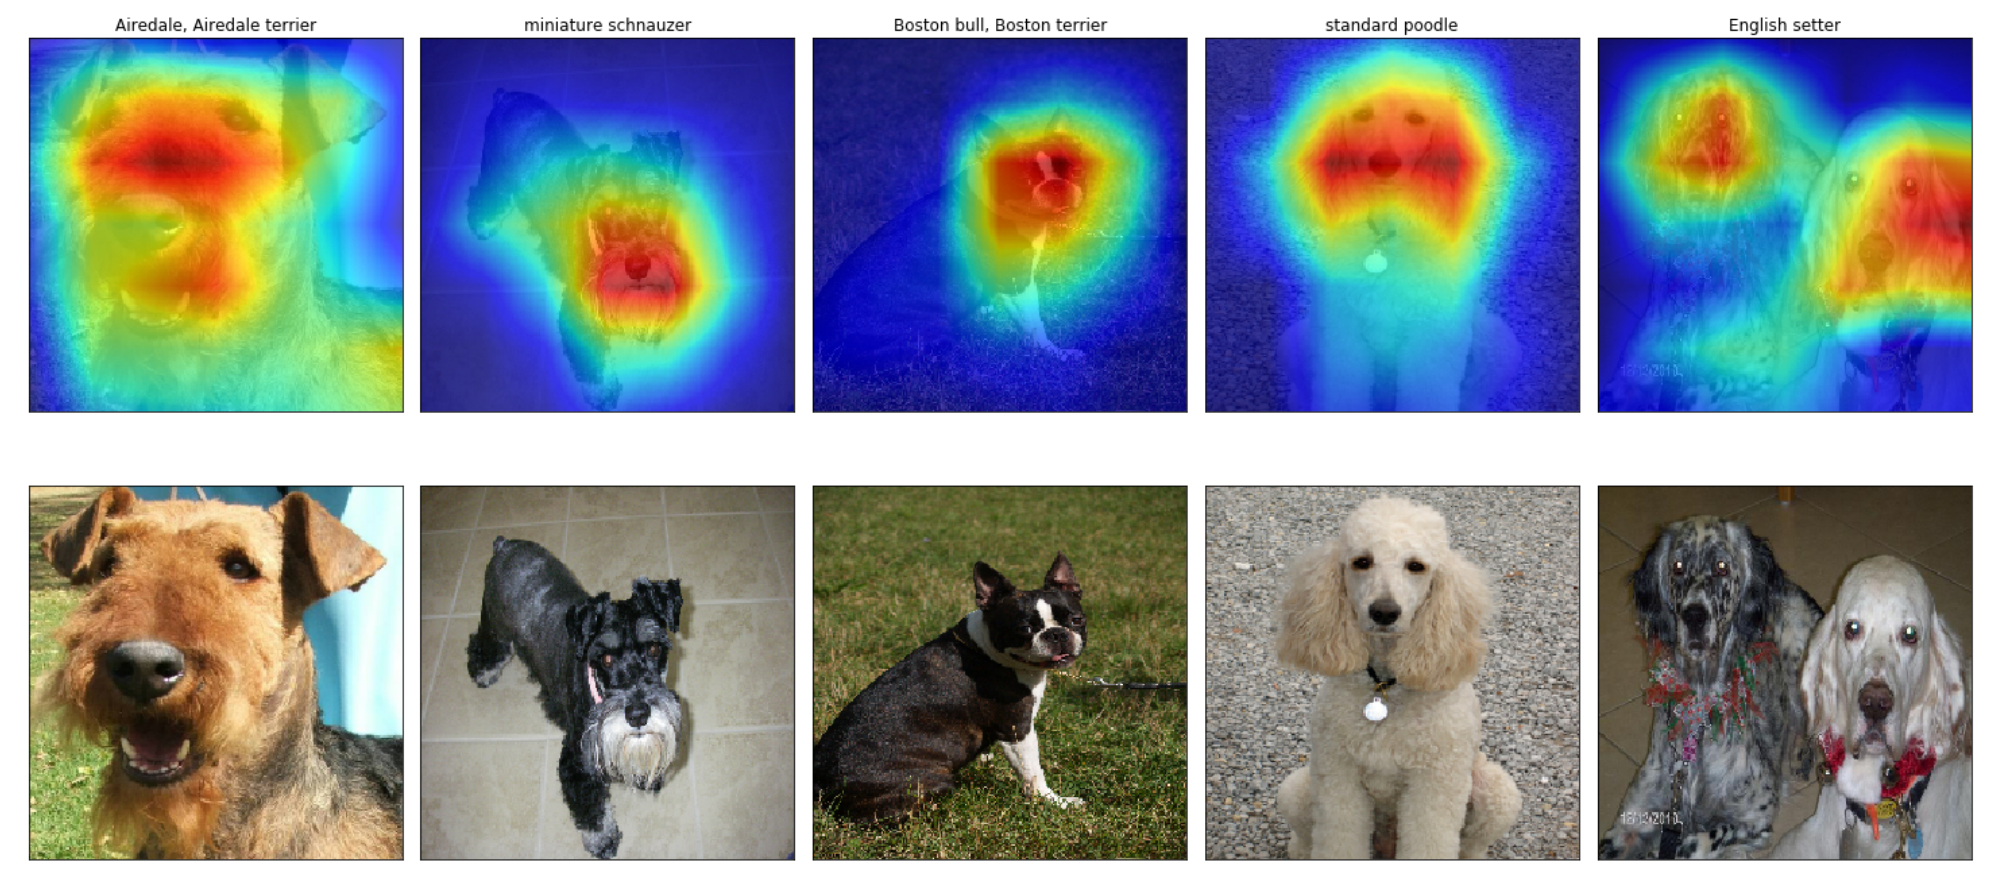
\includegraphics[width=0.9\linewidth]{activation_maps} \\
		\end{center}
	\end{columns}
\end{frame}

%% Person identification
\subsection{Person identification}
\begin{frame}
	\frametitle{Person identification}
	\begin{columns}
		\column{0.45\textwidth}
%		\vspace{-0.2cm}
		\begin{itemize}
			\item Facial landmarks detectors \cite{dlib_review}.
			\vspace{2cm}
			\item Identification according to the color histogram \cite{color_id}.
			\vspace{1cm}
			\item Neural approach: face encoders \cite{facenet}.
%			\vspace{0.8cm}
		\end{itemize}
		
		\column{0.55\textwidth}
		\begin{center}
			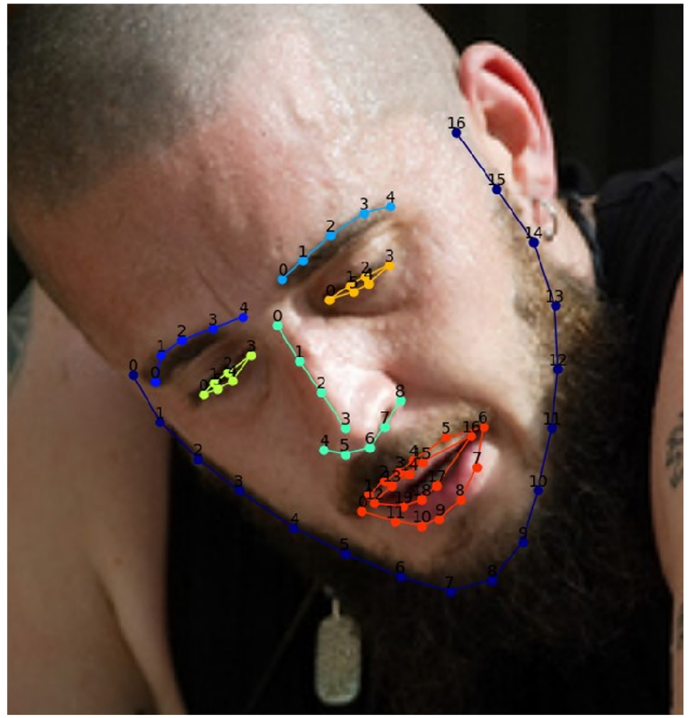
\includegraphics[width=0.45\linewidth]{dlib_landmarks} \\
			\vspace{0.2cm}
			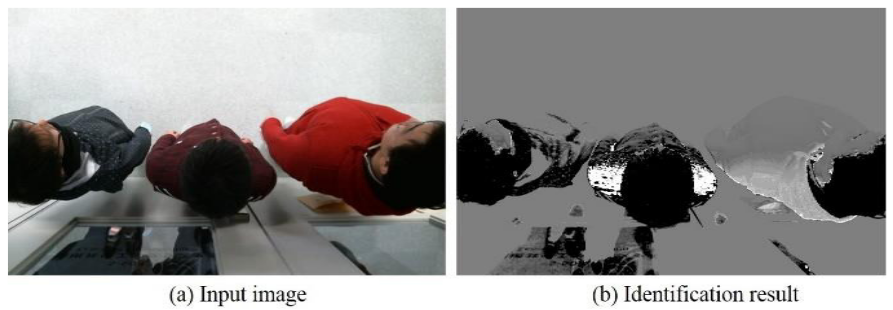
\includegraphics[width=0.9\linewidth]{color_id} \\
			\vspace{0.4cm}
			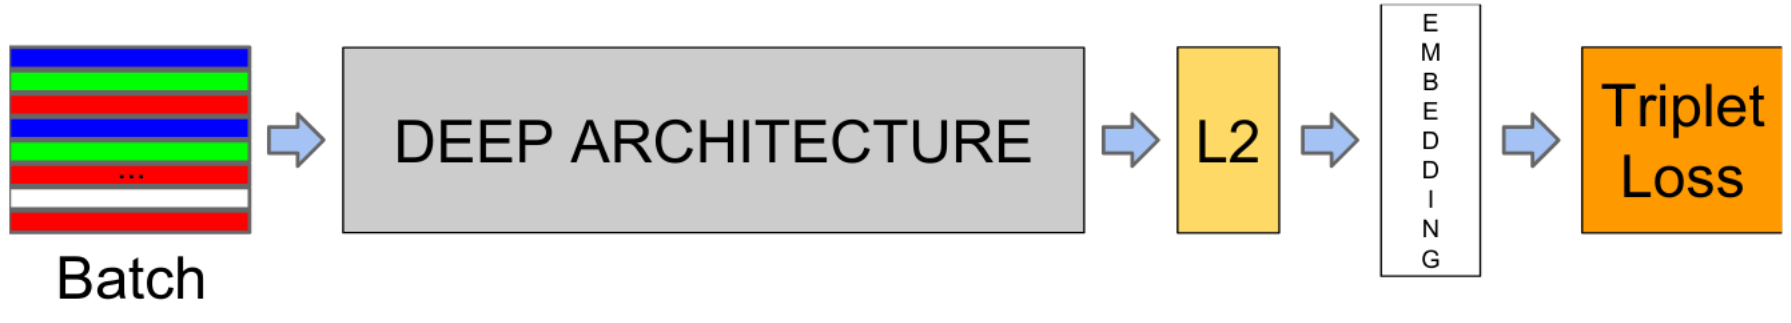
\includegraphics[width=0.95\linewidth]{facenet} \\
			
		\end{center}
	\end{columns}
\end{frame}

%% Embedded deployment
\subsection{Embedded deployment}
\begin{frame}
	\frametitle{Embedded deployment}
	\begin{columns}
		\column{0.5\textwidth}
		%		\vspace{-0.2cm}
		\begin{itemize}
			\item Mounting a laptop.
			\vspace{2cm}
			\item Portable board (Arduino, Raspberry Pi).
			\vspace{1cm}
			\item Embedded computer (NVIDIA Jetson).
		\end{itemize}
		
		\column{0.5\textwidth}
		\begin{center}
			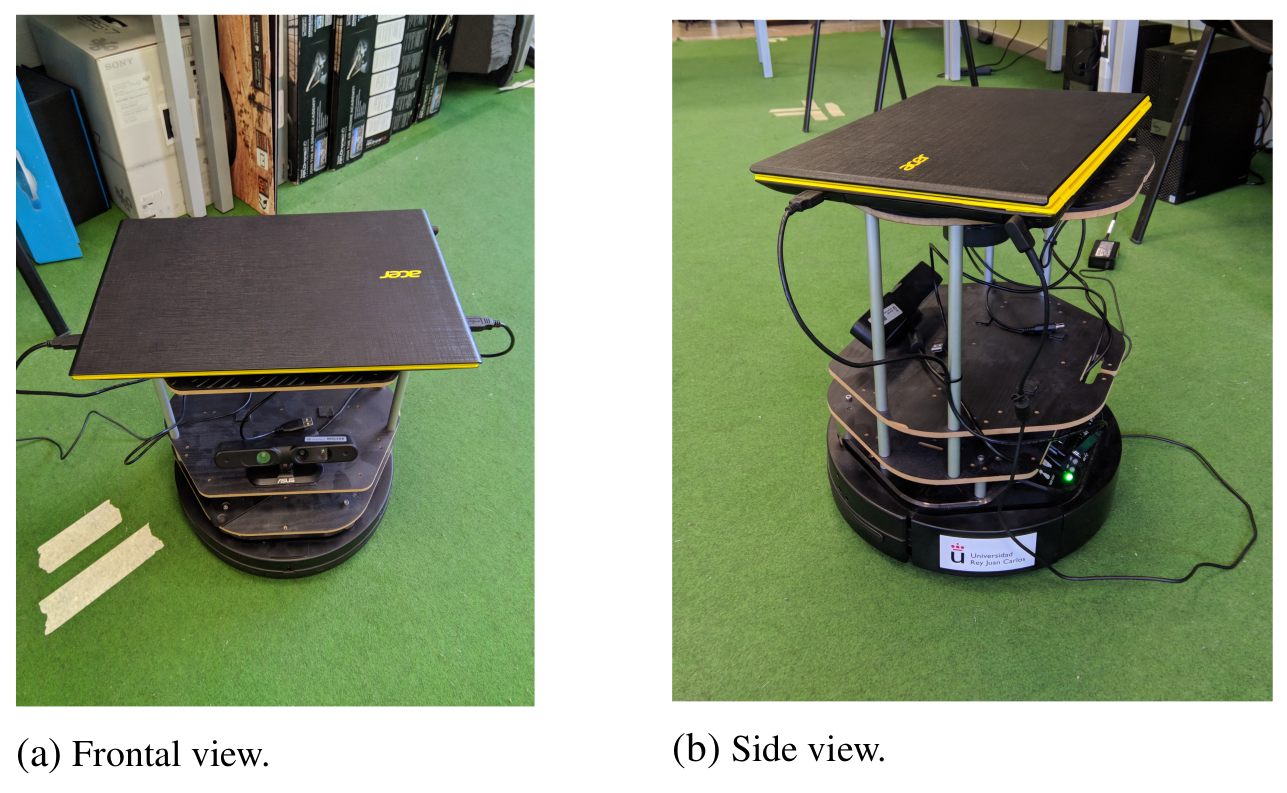
\includegraphics[width=0.6\linewidth]{robot_tfg} \\
			\vspace{0.2cm}
			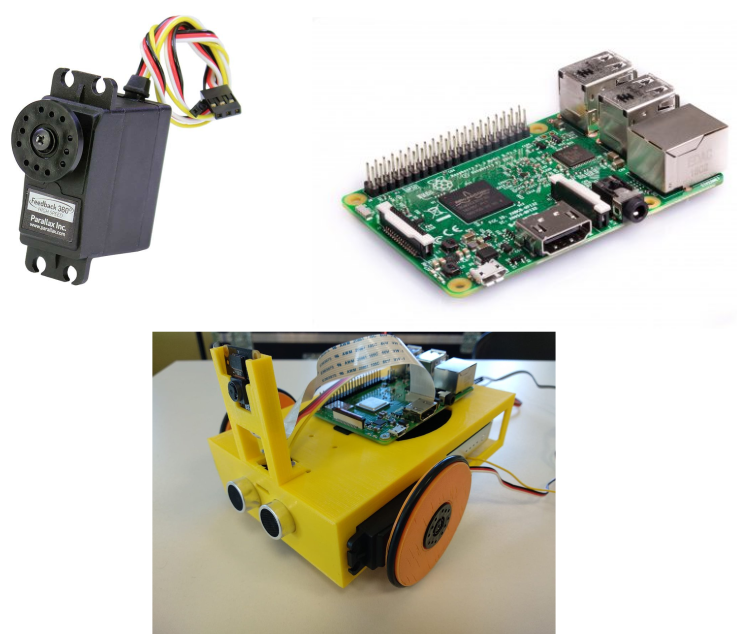
\includegraphics[width=0.55\linewidth]{pibot} \\
			\vspace{0.4cm}
			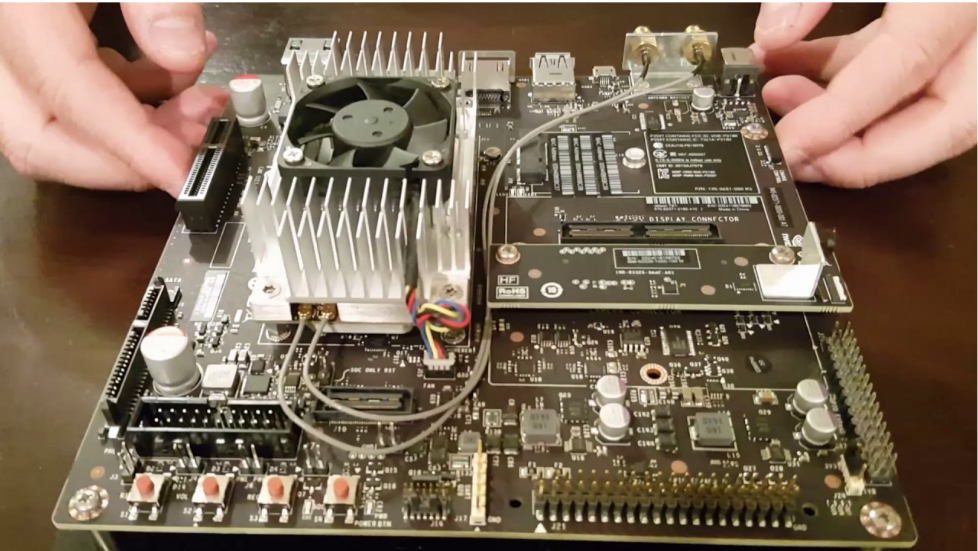
\includegraphics[width=0.6\linewidth]{tx2} \\
			
		\end{center}
	\end{columns}
\end{frame}

%% Following behavior
\subsection{Following behavior}
\begin{frame}
	\frametitle{Following behavior}
	\begin{columns}
		\column{0.5\textwidth}
		%		\vspace{-0.2cm}
		\begin{itemize}
			\item Computing a path towards the person \cite{personfollowing_summary}.
			\vspace{2cm}
			\item Reactive following \cite{personfollowing_reactive}.
		\end{itemize}
		
		\column{0.5\textwidth}
		\begin{center}
			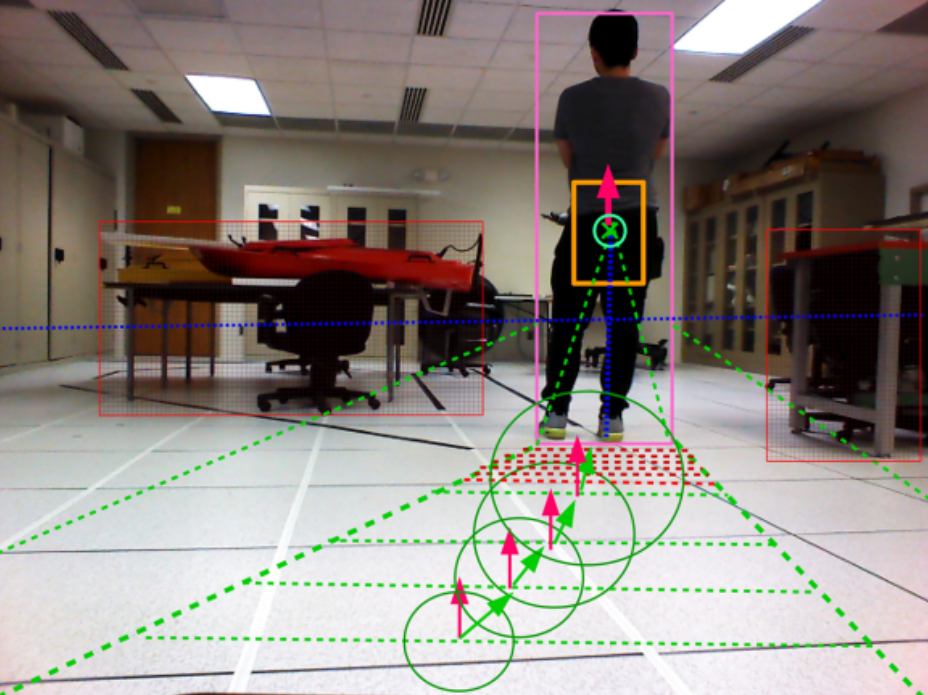
\includegraphics[width=0.8\linewidth]{following_planning} \\
			\vspace{0.2cm}
			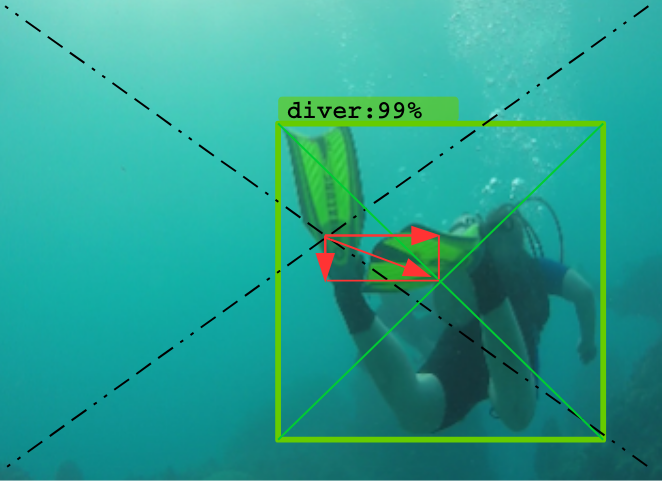
\includegraphics[width=0.8\linewidth]{following_reactive} \\
			
		\end{center}
	\end{columns}
\end{frame}


% Proposed solution
\section{Proposed solution}
% Resources (HW + SW)
\subsection{Resources}
\begin{frame}
	\frametitle{Resources}
\end{frame}
\subsection{Design}
\begin{frame}
	\frametitle{Perception Module}
\end{frame}

\begin{frame}
	\frametitle{Actuation Module}
\end{frame}

\section{Results}
\begin{frame}
	\frametitle{Person detection}
\end{frame}

\begin{frame}
	\frametitle{Face detection}
\end{frame}

\begin{frame}
	\frametitle{Face recognition}
\end{frame}

\begin{frame}
	\frametitle{TensorRT Optimizations}
\end{frame}

\begin{frame}
	\frametitle{Motion tracker}
\end{frame}

\section{Conclusions}

% BIBLIOGRAPHY
\begin{frame}[allowframebreaks]
	\frametitle{References}
	\bibliographystyle{amsalpha}
	\bibliography{bibliography/bibliography.bib}
\end{frame}

\end{document}